%% Vorlage Bachelorarbeit

%% Versionshistorie:

%% v1.0: Erstellung durch Johannes Woske, IT2010, j.woske+latex@gmail.com
%% v2.0: Überarbeitung und Ergänzung durch Anne Traulsen, IT2015, a.traulsen+latex@gmail.com

\documentclass[
	12pt, %Schriftgröße
	a4paper,
	listof=totoc, %Inhaltsverzeichniseinträge für Listen (z.B. Abbildungen)
	bibliography=totoc, %Inhaltsverzeichniseinträge f+r Quellen
	numbers=noenddot, %Entfernt Punkt hinter Gliederungsnummern
	ngerman, %Sprachpaket
	headsepline, %Headertrennlinie
	%footsepline, %Footertrennlinie
	oneside %einseitiges Druckformat %%% Unterdrücken der leeren Seite nach Titelblatt
	]{scrbook} %Dokumentenklasse (Koma-Script)
\usepackage[section]{placeins}
\usepackage[T1]{fontenc}
\usepackage{float}
\usepackage[utf8]{inputenc}
\usepackage[ngerman]{babel}
\usepackage{url}
\usepackage{graphicx} %Bilder einfügen
%\usepackage{pdfpages} %PDF einfügen
\usepackage[a4paper, margin=1in]{geometry}
\usepackage[right]{eurosym} %Euro-Zeichen
\usepackage{amssymb}
\usepackage{cite} %Quellenangaben
\usepackage{setspace} % Zeilenabstand
\usepackage[ 
   colorlinks,        % Links ohne Umrandungen in zu wählender Farbe 
   linkcolor=black,   % Farbe interner Verweise 
   filecolor=black,   % Farbe externer Verweise 
   citecolor=black,   % Farbe von Zitaten 
   urlcolor=blue	  % Farbe von Links
   ]{hyperref} %Verlinkungen
\usepackage{bookmark}
\usepackage[figure]{hypcap}
\usepackage[ngerman]{translator}
\usepackage{blindtext} % Lorem-Ipsum-Plugin
\usepackage{scrhack}
%\usepackage[
	%nonumberlist, %keine Seitenzahlen anzeigen
	%acronym,      %ein Abkürzungsverzeichnis erstellen
	%toc,          %Einträge im Inhaltsverzeichnis
	%section      %im Inhaltsverzeichnis auf section-Ebene erscheinen
	%]
%{glossaries}
\usepackage{outlines}

\usepackage{listings,xcolor} %Codeanzeige
\usepackage[normalem]{ulem}
\useunder{\uline}{\ul}{}


\usepackage{mathtools}
\DeclarePairedDelimiter\abs{\lvert}{\rvert}%
\DeclarePairedDelimiter\norm{\lVert}{\rVert}%
% Swap the definition of \abs* and \norm*, so that \abs
% and \norm resizes the size of the brackets, and the 
% starred version does not.
\makeatletter
\let\oldabs\abs
\def\abs{\@ifstar{\oldabs}{\oldabs*}}
%
\let\oldnorm\norm
\def\norm{\@ifstar{\oldnorm}{\oldnorm*}}
\makeatother

\usepackage{chngcntr}
\counterwithout{figure}{chapter}
\counterwithout{table}{chapter}



%%%%%%%%%%%%%%%%%%%%%%%%%
%%
%% Code Definition
%%
\lstdefinelanguage{powershell}%
  {
	alsodigit = {-},   
   morekeywords={abstract,break,case,catch,const,continue,do,else,elseif,%
      end,export,false,for,function,immutable,import,importall,if,in,%
      macro,module,otherwise,quote,return,switch,true,try,type,typealias,%
      using,while,new-object,psobject,Get-Command,Process,Get-ADUser,Select,ActiveXObject},%
   sensitive=true,%
   alsoother={\$},%
   morecomment=[l]\#,%
   morecomment=[n]{\#=}{=\#},%
   morestring=[s]{"}{"},%
   morestring=[m]{'}{'},%
}[keywords,comments,strings]%

%\lstset{
%	language         = [Sharp]C,
%	basicstyle       = \ttfamily,
%    numbers=left, 
%    numberstyle=\tiny, 
%    numbersep=5pt,
%    breaklines=true,
%    frame=single,
%    escapeinside={(*@}{@*)}, %nicht anzuzeigende Ausdrücke, z.B. für Labels
%    language=sh,
%    basicstyle=\ttfamily\fontsize{10}{12}\selectfont,
%    keywordstyle    = \color{dkblue},
%    stringstyle     = \color{red},
%    identifierstyle = \color{black},
%    commentstyle    = \color{gray},
%    emph            =[1]{php},
%    emphstyle       =[1]\color{black},
%    emph            =[2]{if,and,or,else,Parameter,-Property},
%    emphstyle       =[2]\color{dkyellow},
%    } 

\usepackage{color}
\definecolor{bluekeywords}{rgb}{0,0,1}
\definecolor{greencomments}{rgb}{0,0.5,0}
\definecolor{redstrings}{rgb}{0.64,0.08,0.08}
\definecolor{xmlcomments}{rgb}{0.5,0.5,0.5}
\definecolor{types}{rgb}{0.17,0.57,0.68}

\usepackage{listings}

\lstset{language=csh,
captionpos=b,
%numbers=left, %Nummerierung
%numberstyle=\tiny, % kleine Zeilennummern
frame=single, % Kasten, lines alternativ
showspaces=false,
showtabs=false,
breaklines=true,
showstringspaces=false,
breakatwhitespace=true,
escapeinside={(*@}{@*)},
commentstyle=\color{greencomments},
morekeywords={partial, var, value, get, set},
keywordstyle=\color{bluekeywords},
stringstyle=\color{redstrings},
basicstyle=\ttfamily\small,
captionpos=b,
numbers=left, 
numberstyle=\tiny, 
numbersep=5pt
}

%%%%%%%%%%%%%%%%%%%%%%%%%%%%%%%%%%%%%%%%%%%%%%%%%%%%%
%%%%%%%%%%% Sonderformatierung
%%%%%%%%%%%%%%%%%%%%%%%%%%%%%%%%%%%%%%%%%%%%%%%%%%%%%

% Seitenabstände definieren
\geometry{verbose,tmargin=3cm,bmargin=2cm,lmargin=3cm,rmargin=3cm} 

% Hurenkinder und Schusterjungen verhindern (Ja, das heißt wirklich so!!!)
\clubpenalty = 10000 \widowpenalty = 10000 \displaywidowpenalty = 10000 

\newcommand{\footfigref}[1]{\footnote{Abb. \ref{#1} auf Seite \pageref{#1}}}

%% Bei Referenzen im Text wird jetzt bei allen Ebenen "Kapitel" vorgestellt, z.b. Kapitel 2, Kapitel 2.2, Kapitel 6.3.2
\addto\extrasngerman{%
    \def\sectionautorefname{Kapitel}%
    \def\subsectionautorefname{Kapitel}%
    \def\subsubsectionautorefname{Kapitel}%
    }

% Vertikaler Abstand zwischen Ende Textblock - Ende Fußzeile --> Abstand der Seitenzahl von Rand erhöhen 
\setlength{\footskip}{10mm}

% Abstand vor/nach Überschriften verändern

\RedeclareSectionCommand[%
    beforeskip=0.5\baselineskip,
    afterskip=0.5\baselineskip
]{chapter}

\RedeclareSectionCommand[%
    beforeskip=0.5\baselineskip,
    afterskip=0.5\baselineskip
]{section}

\RedeclareSectionCommand[%
    beforeskip=0.1\baselineskip,
    afterskip=0.1\baselineskip
]{subsection}

\RedeclareSectionCommand[%
    beforeskip=0.01\baselineskip,
    %%afterskip=0.2\baselineskip
]{paragraph}

\usepackage[acronym, nonumberlist]{glossaries} %% use after hyperref %Glossar-Paket laden


\setlength{\abovecaptionskip}{4pt}  % 1pc=12pt 
\setlength{\belowcaptionskip}{0pt}
%\setlength{\textfloatsep}{4pt}
\setlength{\intextsep}{1pc}

%% Verkleinerung der Textgröße unter Abbildungen
\addtokomafont{caption}{\small}

% falsche Default-Silbentrennung überschreiben
%falsche Default-Silbentrennung überschreiben
\hyphenation{Soft-ware-ent-wick-lung}

% Den Punkt am Ende der Glossareinträge deaktivieren
\renewcommand*{\glspostdescription}{}

%Glossar-Befehle anschalten
%\makeglossaries
\loadglsentries{glossar.tex}
\makenoidxglossaries 

% sorgt dafür, dass bei Leerzeile die Einrückung verhindert und stattdessen eine Leerzeile eingefügt wird % erspart bigskips und erhöht die Lesbarkeit im LaTeX-Text 
\KOMAoptions{parskip=full*}

% ändert Titelschriftart in Serifen-Normalschriftart
\addtokomafont{disposition}{\rmfamily} 





%%%%%%%%%%%%%%%%%%%%%%%%%%%%%%%%%%%%%%%%%%%%%%%%%%%%%
%%%%%%%%%%% Textbausteine
%%%%%%%%%%%%%%%%%%%%%%%%%%%%%%%%%%%%%%%%%%%%%%%%%%%%%
%%%%%%%%%%%% Studentennamen
\newcommand{\studentNameEins}{Jahn, Marko}
\newcommand{\studentNameZwei}{Schenkewitz, Mario}
\newcommand{\studentNameDrei}{Zilius, Sven}
%%%%%%%%%%%% Typ der Arbeit
\newcommand{\type}{Studienprojekt I}
%%%%%%%%%%%% Thema
\newcommand{\topic}{Schatzinsel}
%%%%%%%%%%%% Untertitel
\newcommand{\subtopic}{Entwickeln eines Spiels durch objektorientiertes Programmieren}
%%%%%%%%%%%% Studienbereich
\newcommand{\studienbereich}{Technik}
%%%%%%%%%%%% Fachrichtung
\newcommand{\fachrichtung}{Duales Studium Wirtschaft • Technik}
%%%%%%%%%%%% Studiengang
\newcommand{\studiengang}{Informatik}
%%%%%%%%%%%% Betrieb
\newcommand{\company}{}
%%%%%%%%%%%% Betreuer HWR
\newcommand{\betreuerHS}{Zimmermann, Arthur}
%%%%%%%%%%%% Betreuer Unternehmen
\newcommand{\betreuerUnt}{}
%%%%%%%%%%%% Jahrgang
\newcommand{\jahrgang}{2020}
%%%%%%%%%%%% Matrikelnummer
\newcommand{\MatrEins}{612678}
\newcommand{\MatrZwei}{685593}
\newcommand{\MatrDrei}{696087}
%%%%%%%%%%%% Modul
\newcommand{\Modul}{IT3161, Studienprojekt I}
%%%%%%%%%%%% Anzahl Wörter
\newcommand{\wordsnr}{TDB}
%%%%%%%%%%%% Fertigstellungsdatum
\newcommand{\Dateofcompletion}{TBD}
%%%%%%%%%%%%%%%%%%%%%%%%%%%%%%%%%%%%%%%%%%%%%%%%%%%%%>>>>>>>


\begin{document}

%%%%%%%%%%%%%%%%%%%%%%%%%%%%%%%%%%%%%%%%%%%%%%%%%%%%%>>>>>>>
%%%%%%%%%%% Titelblatt

%% Anordnung und Aussehen von Titel und Untertitel

\subject{\type}

\title{
\normalfont\endgraf\rule{\textwidth}{.4pt}
\begingroup
	\centering
	\linespread{1.5}
	\huge\topic
\endgroup
\linespread{1}
\ \\ % Falls kein Subtopic, auskommentieren
\ \\ % Falls kein Subtopic, auskommentieren
\large\subtopic % Falls kein Subtopic, auskommentieren
\endgraf\rule{\textwidth}{.4pt}
}
 
%%Eigentlich nicht besonders schön, aber Koma erlaubt die Anordnung eines weiteren Felden (hier: Fachbereich) nicht
\date{\normalsize fertiggestellt am \Dateofcompletion \\ \textbullet \\ Fachbereich Duales Studium Wirtschaft / Technik \\
Hochschule für Wirtschaft und Recht Berlin}
%% \date muss leer angegeben werden, um die Default-Datumsanzeige zu unterdrücken

\publishers{
	\begin{tabular}{l l}
	\textbf{\normalsize{}} & \normalsize{}  \tabularnewline
	%\textbf{\normalsize{}} & \normalsize{}  \tabularnewline
	\textbf{\normalsize{Name:}} & \normalsize{\studentNameEins, \MatrEins} \tabularnewline
	\textbf{\normalsize{Name:}} & \normalsize{\studentNameZwei, \MatrZwei} \tabularnewline
	\textbf{\normalsize{Name:}} & \normalsize{\studentNameDrei, \MatrDrei} \tabularnewline
	\textbf{\normalsize{Fachrichtung:}} & \normalsize{\fachrichtung} \tabularnewline
	\textbf{\normalsize{Studiengang:}} & \normalsize{\studiengang} \tabularnewline
	\textbf{\normalsize{Studienjahrgang:}} & \normalsize{\jahrgang} \tabularnewline
	\textbf{\normalsize{Betreuer HS:}} & \normalsize{\betreuerHS} \tabularnewline
	\textbf{\normalsize{Anzahl der Wörter:}} & \normalsize{\wordsnr}\\
	
%	\normalsize Vom Betreuer zur Kenntnis genommen:\vspace{2em}\\
%	\end{tabular}
%	\normalsize
%	\begin{tabular}{lp{10em}l} 
% 	\hspace{1cm}   && \hspace{4cm} \\\cline{1-1}\cline{3-3} 
% 	Ort, Datum     && \betreuerHS
	\end{tabular}
	}

\titlehead{\begin{center}
    
\includegraphics[scale=1]{bilder/HWR-Logo.jpg}
    \end{center}
    }

\maketitle

\onehalfspacing % anderthalbfacher Zeilenabstand


%%%%%%%%%%%%%%%%%%%%%%%%%%%%%%%%%%%%%%%%%%%%%%%%%%%%%%%%%%%%%%%%%%%%%%%%%%%%%%%%%%%%%%%%%%%%%%%%%%%%%%%%%%%%%%%%%%%%%%%%%%%
%%%%%%%%%%% Dokumenteninhalt START
%%%%%%%%%%%%%%%%%%%%%%%%%%%%%%%%%%%%%%%%%%%%%%%%%%%%%%%%%%%%%%%%%%%%%%%%%%%%%%%%%%%%%%%%%%%%%%%%%%%%%%%%%%%%%%%%%%%%%%%%%%%

%%%%%%%%%%%%%%%%%%%%%%%%%%%%%%%%%%%%%%%%%%%%%%%%%%%%%
%%%%%%%%%%% Abstract
\chapter*{Abstract}
\addcontentsline{toc}{chapter}{Abstract}
Development of games isn't for entertainment Purposes only nowadays. It is possible do model different environments and worlds through them and to use those for simulations or predictions.
In light of this it is evaluated how well suited older and modern development Environments are in realizing these games.
The scenario of a Treasure Island serves as an example. Pirates on this island move in random directions and let each other know when the treasure is located.  
In this Paper Java, Unreal Engine and Unity Engine are considered for the making of this game.

\pagenumbering{Roman} % römische Seitenzahlen

\chapter*{Kurzfassung}
\addcontentsline{toc}{chapter}{Kurzfassung}
Die Entwicklung von Spielen ist Heutzutage nicht nur für Unterhaltungszwecke interessant. Es ist möglich durch sie auch verschiedene Umgebungen und Welten modellieren und für Simulationen oder vorhersagen verwenden. Vor diesem Hintergrund wird untersucht, wie ältere und moderne Entwicklungsumgebungen sich eignen in der Umsetzung von Spielen.  
Als Beispiel dient das Szenario einer Schatzinsel, auf der Piraten einen Schatz suchen. Sie Bewegen sich in zufällige Richtungen und lassen sich gegenseitig wissen, wenn der Schatz gefunden wurde.
Betrachtet werden in dieser Arbeit die Umsetzung in Java, Unreal Engine und Unity Engine.

%%%%%%%%%%%%%%%%%%%%%%%%%%%%%%%%%%%%%%%%%%%%%%%%%%%%%
%%%%%%%%%%% Inhaltsverzeichnis, Tabellen, Abbildungen, etc.
\newpage

\tableofcontents{}
\addcontentsline{toc}{chapter}{Inhaltsverzeichnis}

\listoffigures
%\listoftables

%\section*{Hinweis}
%
%Aus Gründen der besseren Lesbarkeit wird im Text verallgemeinernd die weibliche Form verwendet. Diese Formulierungen umfassen gleichermaßen weibliche und männliche Personen.
%\clearpage

\addcontentsline{toc}{chapter}{Akronyme}
\printnoidxglossaries

\clearpage

%% arabische Seitenzahlen
\pagenumbering{arabic}

%%%%%%%%%%%%%%%%%%%%%%%%%%%%%%%%%%%%%%%%%%%%%%%%%%%%%
%%%%%%%%%%% Einführung

\chapter{Einleitung}\label{sec:einleitung}
Die \gls{OOP} ist ein heutzutage weit verbreitetes Computerprogrammiermodell oder Programmierparadigma. In der \gls{OOP} werden Anwendungen um so genannte Objekte und deren Daten herum strukturiert und nicht um Funktionen oder Logik. So fokussiert sich die \gls{OOP} auf Objekte, mit denen eine Anwendung interagiert, diese Objekte können als Datenfeld mit Attributen und eigenem Verhalten angesehen werden.

Einen tieferen Einblick in das Thema der \gls{OOP} soll der Abschnitt \ref{sec:Grundlagen} bieten, in dem die Basis für die \gls{OOP} näher erörtert wird.

Thema dieses Studienprojektes ist es sich dieses Programmierparadigma zunutze zu machen, um ein Spiel zu entwickeln.\\
Der Titel des Spiels ist \glqq Schatzinsel\grqq, es handelt von drei Piraten, die sich auf einer Insel befinden, auf der ebenfalls ein Schatz versteckt ist. Es ist ihnen unbekannt wo sich dieser Schatz befinden. Durch zufällige Bewegung über die Insel wollen sie versuchen diesen Schatz zu finden. Jeder der Piraten hat verschiedene Eigenschaften, wie zum Beispiel Geschwindigkeit.\\
Sobald einer der Piraten den Schatz entdeckt, ruft er die anderen zu sich. Am Ende versammeln sie sich alle um den Schatz.

Dieser Umstand soll durch das Spiel modelliert und gegebenenfalls erweitert werden.

\chapter{Grundlagen}\label{sec:Grundlagen}
\section{Objektorientierte Programmierung}
\gls{OOPL} eignen sich durch die Konzentration auf die Objekte, mit denen das Programm interagieren soll, dazu, dass Software Wartbar und lesbar bleibt. Objekte und ihre Methoden können getrennt voneinander erstellt und programmiert werden. Diese Unterteilung in Einzelteile ermöglicht des Weiteren die Wiederverwendbarkeit von Code, also dem Quelltext, entweder in dem die Klasse selbst wiederverwendet wird, oder eine andere Klasse von ihr erbt. Dazu mehr im Abschnitt \ref{sec:Vererbung}

\gls{OOP} ist ein Programmierstil, der mittlerweile in Unternehmen, Industrie und akademischen Kreisen seinen Platz gefunden hat. Es wird ein natürlicheres und dadurch ein mächtigeres Entwurfsparadigma insofern erwartet, dass ein Programmierer produktiver ist, wenn das Anwendungsmodell näher am Problem modelliert werden kann, dass gelöst wird.\\
Anders gesagt ist eine \gls{OOPL} mächtiger, weil es einem Programmierer erlaubt ein Problem zu lösen, dass die Struktur einer Welt nachbildet, in welcher das Problem entstand. Vertrautheit mit solch einer Sprache eröffnet Wege zu einer klaren und natürlichen Lösung \cite{OOPL}.

Es werden also im betrachteten Fall der Schatzinsel die Objekte, die aus der echten Welt bekannt sind, so modelliert, dass die Interaktionen und Verhaltensweisen natürlich in einer Anwendung modelliert werden können.

\section{Datenabstraktion und Verkapselung}
Einer der ersten Schritte bei der \gls{OOP} ist es alle Objekte zu sammeln, die manipuliert werden müssen. Im Fall des Spiels \glqq Schatzinsel\grqq \hspace{0.1cm}gibt es zum Beispiel Piraten, eine Insel, ein Schatz, aber auch eine graphische Benutzeroberfläche die alle als Objekt betrachtet werden können. Sie müssen untereinander aber auch mit dem Benutzer interagieren können.

Einer der großen Durchbrüche bei der Gestaltung von Programmiersprachen geschah, als es ermöglicht wurde, dass Programmierer eigene Datentypen definieren konnten. C.A.R. Hoare's record class in Simula67 gilt als die Quelle der Idee.\cite{OOPL}
Verbreitung des, durch Programmierer definierten, Datentyps fand durch die Sprache Pascal statt. \cite{Pascal}

So kann in Pascal ein Verbund definiert werden, der selbst aus Daten besteht, siehe Listing \ref{lst:record1}. 

\begin{lstlisting}[language=Pascal, caption=Verbund Beispiel Definition \cite{PascalVerbund}, label={lst:record1}]
TYPE Auto = RECORD
KFZ: String[12];
Gewicht: Real;
AnzPassagiere: Integer;
END;
\end{lstlisting}

Dieses Beispiel (Listing \ref{lst:record2}) definiert einen neuen Datentyp \textit{Auto}, in dem jeweils die Art des KFZ, das Gewischt und die Anzahl der Passagiere angegeben wird. Nun kann man den Typen \textit{Auto} nutzen, um beliebig viele Daten-Entitäten zu erstellen.

\begin{lstlisting}[language=Pascal, caption=Verbund Beispiel Instantiierung \cite{PascalVerbund}, label={lst:record2}]
VAR a : Auto;
BEGIN
a.KFZ := 'B XY 123456';
a.Gewicht := 555.77;
a.AnzPassagiere := 5;
END;
\end{lstlisting}

Manipulationen der Daten innerhalb des Verbunds werden extern vom Datentyp selbst betrachtet, die Syntax der Sprache indiziert somit nur eine Gruppierung von Daten.

Verbunde in Pascal werden homogen genannt, wenn alle Daten innerhalb des Verbunds denselben Typ haben. Sie sind heterogen, wenn es verschiedene Typen, wie im Beispiel, gibt.

Pascal erlaubt zwar die Erstellung von heterogenen Verbunden, jedoch ist es nicht möglich in diesen Verbunden Operationen einzubauen. Anders als bei Pascal ist die bei Java zum Beispiel möglich.  

\begin{lstlisting}[language=Java, caption=Operation innerhalb einer Klasse \cite{OOPL}, label={lst:Java-Operation}]
class Point {
private int x, y;
	public int getX() { return x; }
	public int getY() { return y; }
	public void setXY(int x, int y) {
		if (x >= 0 && y >= 0) {
			this.x = x;
			this.y = y;
		}
	}
}
\end{lstlisting}

Im Listing \ref{lst:Java-Operation} wird zum Beispiel durch die Funktion \glqq setXY()\grqq{} ermöglicht, dass x und y gesetzt werden können. Es ist zu bemerken, dass verschiedene Sichtbarkeiten gesetzt werden. Dadurch, dass x und y auf \emph{private} gesetzt sind, können sie also von außen nur durch die Funktion \glqq setXY()\grqq{} geändert werden.  
Dies veranschaulicht auch das Konzept der Verkapselung \cite{OOPL} Seite 4.  

Datenabstraktion in ihrer vollen Kapazität beschreibt also die Möglichkeit für Programmierer ihre eigenen Datentypen zu definieren, diese Typen können eine Heterogene Struktur haben und die Sicht auf diese kann eingeschränkt werden. Außerdem ist es möglich Operationen innerhalb dieser Datentypen zu haben.  

In diesem Zusammenhang kann gesagt werden, dass Objekte also aus Attributen und Operationen, auch Funktionen oder Methoden genannt, bestehen und Instanzen von diesen Datentypen sind. Diese Datentypen werden im Allgemeinen auch als Klassen bezeichnet.


\section{Vererbung}\label{sec:Vererbung}
Die Beziehung zwischen Typen in spielt eine wichtige Rolle in den \gls{OOPL}, so ist die Vergleichbarkeit von Typen wichtig, um Objekte zu vergleichen.  
Diese Beziehungen werden durch Vererbung erweitert und bereichert. Es stellt sich ein System aus Vererbungs- und Subtypenbeziehungen dar, diese Tragen zur Komplexität einer Sprache bei. Dabei spielen verschiedene Begriffe zentrale Rollen.  
Zum Beispiel wird gesagt, dass Klasse B von Klasse A \emph{erbt} oder \emph{abgeleitet} ist, wenn Objekte der Klasse B mindestens dieselben Attribute und Verhaltensweisen wie Objekte der Klasse A haben. Die Objekte der Klasse B können auch mit eigenen Attributen und Methoden erweitert werden.  
B \emph{erbt} diese Attribute von A. Dann ist A die \emph{Basisklasse}, manchmal auch als \emph{Elternklasse} bezeichnet, von der B abgeleitet wird.  
Im englischen werden oft auch die Begriffe \emph{Superklass} (Oberklasse) und \emph{Subclass} (Unterklasse) verwendet.  
Subtypenbeziehungen gestalten sich ähnlich zur Vererbung. Damit eine Subtypenbeziehung besteht, müssen Objekte des Typs B auch als Objekte des Typs A gelten. Nicht nur die Attribute des Objekts vom Typ B stimmen mit denen vom Typ A überein, auch die Zugriffsrechte und Sichtbarkeit auf die verschiedenen Attribute müssen übereinstimmen. Das heißt, dass alle Attribute und Methoden, die in Typ A zur Verfügung stehen, auch in Typ B zur Verfügung stehen.  
Wenn diese Bedingung erfüllt ist, dann können auch immer Objekte vom Typ B als Argumente an Parameter des Typen A gegeben werden. Im englischen wird gesagt B ist ein \emph{subtype} (Untertyp) von A beziehungsweise A ist ein \emph{supertype} (Obertyp) von Typ B. Im Allgemeinen ist es so, dass es immer, wenn die Funktionalität der Vererbung gegeben ist, auch immer die Funktionalität für Subtypen in Programmiersprachen existiert.  
  
Ein Datentyp, der Vererbung eingearbeitet hat, wird auch als Klasse bezeichnet (s.O.).

\begin{lstlisting}[language=Java, caption=Erweiterung der Point Klasse aus Listing \ref{lst:Java-Operation} \cite{OOPL}, label={lst:Vererbung}]
class Disk extends Point {
	private double radius;
	private Color color;
	public double getRadius() { return radius; }
	public void setRadius(double radius) {
		if (radius > 0) this.radius = radius;
		}
	public Color getColor() { return color; }
	public void setColor(Color color) { this.color = color; }
}
\end{lstlisting}

Im Listing \ref{lst:Vererbung} wird die Klasse \glqq Point\grqq{}  aus \ref{lst:Java-Operation} erweitert. Da eine Scheibe einen Punkt als Basis hat, kann die Klasse auch so erweitert werden, dass man einen Radius und z.B. eine Farbe hinzufügt. Die Vererbung selber ändert nichts an der Verwendung dieser neuen Klasse. Sie muss immer noch Instantiiert werden und über Methoden ihre Parameter gesetzt werden, dafür dienen die Methoden setRadius(), SetColor() und die geerbte Methode setXY(). Es ist also Beispielweise möglich mit den folgenden Befehlen ein entsprechendes Objekt zu erstellen siehe Listing \ref{lst:Instantiierung}.

\begin{lstlisting}[language=Java, caption=Instantiierung der Klasse Disk \cite{OOPL}, label={lst:Instantiierung}]
Disk d = new Disk();
d.setXY(100,210);
d.setRadius(25.7);
d.setColor(Color.red);
\end{lstlisting}

Es ist zu bemerken, dass die Methoden über das Objekt aufgerufen werden. Es gibt die Möglichkeit auch Methoden auszuführen, die über Klassen ausgeführt werden. Solche Methoden nennt man auch statische Methoden, sie werden über das Schlüsselwort \emph{static} im Quelltext der Sprachen Java, C++ und C\# identifiziert.

\section{Polymorphismus}
%Seite 32
Subklassen sind oft spezialisierte Klassen
daher notwendig , dass ein spezialisiertes Objekt ihre Methoden anders ausführt
wir benötigen die Möglichkeit Methoden zu überschreiben \emph{override}

Subklassen sind oft spezialisierte Klassen, die von einer Oberklasse erben. Oft ist es zu erwarten, dass eine solche spezialisierte Klasse sich anders verhält, wenn man eine Methode der Oberklasse aufruft. Man kann zur Veranschaulichung eine Klasse betrachten, die ein beliebiges Tier darstellen soll siehe Listing \ref{lst:Tier}.

\begin{lstlisting}[language=Java, caption=Klasse Tier, label={lst:Tier}]
class Tier
{
    private String name;
    private short alter;
 
    public void gibLaut()
    {
        System.out.println("Geraeusche eines allgemeinen Tiers");
    }

}
\end{lstlisting}

Wenn man nun Unterklassen von der Klasse Tier ableitet, könnte man erwarten, dass die Methode \emph{gibLaut()}, je nachdem, um was für ein Tier es sich handelt, eine andere Ausgabe verursacht.  
Es ist also notwendig eine Möglichkeit zu haben die Verhaltensweisen und Methoden von Oberklassen zu überschreiben. Diese veränderbarkeit der Implementation von Funktionen nennt man auch Polymorphismus. 
So kann man in der Programmiersprache Java mit der Deklaration \emph{\@Override} eine Funktion überschreiben siehe \ref{lst:Katze}.

\begin{lstlisting}[language=Java, caption=Klasse Katze, label={lst:Katze}]
class Katze extends Tier
{
    @Override
    public void gibLaut()
    {
        System.out.println("Miau");
    }
}
\end{lstlisting}

Je nach Sprache ist diese Funktionalität anders implementiert. In der Sprache C++ werden Funktionen, die überschreibbar sein sollen mit dem Schlüsselwort \emph{virtual} gekennzeichnet siehe \ref{lst:TierC++}.

\begin{lstlisting}[language=C++, caption=Tier und Katzen Beispiel in C++, label={lst:TierC++}]
class Tier {
	public:
	virtual char * gibLaut() { return "Geraeusche eines allgemeinen Tiers"; }
	};
	
class Katze : public Tier {
	public:
	char * gibLaut() { return "Miau"; }
};
\end{lstlisting}

\section{Überladen}
Überladen bezieht sich auf Funktionen und Operatoren und bedeutet, dass diese, unter der Verwendung des gleichen Namens, in Abhängigkeit der Typen der übergebenen Parameter verschieden ausgeführt werden. Betrachtet man zum Beispiel die Addition als Operator, so wird bei der Berechnung der Summe von zwei Zahlen je nach Typ der Zahlen die Operation anders ausgeführt.  
Wenn man Zahlen von verschiedenen Typen addieren möchte, dann wird oft impliziert eine Umwandlung der Typen vollzogen. Zum Beispiel wenn eine ganze Zahl mit einer Fließkommazahl addiert wird, dann wird die ganze Zahl in eine Fließkommazahl umgewandelt, bevor sie addiert werden.  
Der + Operator für die Addition wird in einigen Sprachen auch so überladen, dass mit ihm Text verkettet werden kann.  
  
Es ist Programmierern somit auch möglich selber Operatoren oder Funktionen zu überladen.

\chapter{Umgebungen}\label{sec:Umgebungen}
\section{Java Swing}
Java Swing ist eine \gls{GUI} Bibliothek für Java. Es gehört zu den Java Foundation Classes, eine Sammlung von Bibliotheken für dir Programmierung von graphischen Benutzerschnittstellen. Andere Bibliotheken in dieser Sammlung sind zum Beispiel Java 2d, Java Accessibility API, Drag-and-Drop-API und das Abstract Window Toolkit (AWT) \cite{JFC}. Swing baut auf AWT auf und ist mit den anderen APIs verwoben.  
Es gibt auch Konkurrenten zu Swing, z.B. das für Eclipse entwickelte SWT. Auf dieses wird aber nicht eingegangen, da Swing auch mit anderen Entwicklerwerkzeugen und -umgebungen Kompatibel ist.  
Swing ist, im Gegensatz zu AWT, Plattformunabhängig. Außerdem ist es modular und objektorientiert aufgebaut. Die Plattformunabhängigkeit wird dadurch gewährleistet, dass alle Swing-Komponenten direkt von Java gerendert werden. Nachteil davon ist, dass Swing Anwendungen nicht wie Anwendungen aussehen, die nativ auf dem darunterliegenden Betriebssystem entwickelt wurden.  
Es gibt so genannte \glqq Look-and-Feels\grqq{}, die das Aussehen und Verhalten modifizieren.

\section{Unreal Engine}

Unreal Engine ist eine der am weitesten verbreiteten und fortschrittlichen 3D Entwicklungsumgebungen. Sie wird unter anderem für das Aufnehmen von Animationsfilmen, Präsentationen von Prototypen und zur Erstellung von Computerspielen verwendet.
Für das Programmieren können entweder Blueprints, Unreal`s eigene visuelle Programmiersprache oder C++ verwendet werden. Ein fertiges Projekt wird am Ende für das entsprechende Zielsystem ausgeliefert. Unreal unterstützt hierbei alle verbreiteten Plattformen wie Windows, Mac, Linux und Android.


\section{Unity Engine}
Die Unity Engine ist eine weitverbreitete Entwicklungsumgebung zur Entwicklung von Spielen, aber auch zur Darstellung und Simulation von z.B. Architekturprojekten oder anderer 3D- Modellierungen, sowie zur Produktion von Filmen. Neben der 3D- Modellierung unterstützt Unity auch 2D Projekte in vollem Umfang. Die Entwicklung in Unity erfolgt primär im eigenen Editor, dieser bietet viele Möglichkeiten, um die Programmierung so einfach wie möglich zu halten. Die Entwicklung erfolgt hauptsächlich in C\#. Unity ermöglicht zudem auch eine erleichterte Wiederverwendung von Objekten als \glqq Prefabs\grqq , welche alle Attribute wie Modelle, aber auch alle eingebundenen Skripte gleich wiederzuverwenden. Unity unterstützt neben allen Betriebssystemen auf dem PC auch Android, sowie eine Vielzahl an Konsolen. 

\chapter{Verwendete Werkzeuge}
\section{Git und Github}
Git ist eine Software. Sie dient zur Verwaltung von Versionen beziehungsweise der Versionskontrolle von Projekten. Es wird ermöglicht zu alten Versionen zurückzukehren, Veränderungen zu vergleichen und dient auch als Werkzeug für die Zusammenarbeit von mehreren Personen am selben Projekt.  

Git kann auf verschiedene Arten und Weisen verwendet werden, so kann es über die Kommandozeile, in Github Desktop oder mit einem Git-Klienten ausgeführt werden.

Es werden alle Dateien und Änderungen innerhalb eines Projektordners erfasst und festgehalten, um dadurch nun die Zusammenarbeit zu ermöglichen wird noch eine weitere Plattform benötigt.  
Ein Dienst dient als Host der Projekte auf dem der gesamte Quellcode und alle notwendigen Dateien gespeichert werden. Wir haben für dieses Projekt GitHub gewählt.

GitHub ermöglicht es nun gespeicherte Projekte mit anderen Benutzern zu teilen und sie zu Klonen. Arbeiten mehrere Personen am selben Projekt, so wird beim Hochladen der Änderungen auf den gewählten Dienst verglichen auf welchem Stand sich das Projekt befindet und automatisch verglichen, ob Neuerungen auf der vorhandenen version basieren oder ob sie auf einer älteren Version vorgenommen wurden.  

Wenn Aktualisierungen des Projekts gab, dann bietet Git die Möglichkeit, Konflikte zu beseitigen, um die verschiedenen Versionsstände zu vereinen.

Git bietet noch viele weitere Funktionen, die die Zusammenarbeit erleichtern und fördern, die in diesem Dokument nicht näher behandelt werden.

\section{Eclipse}
Eclipse ist eine integrierte Entwicklungsumgebung die hauptsächlich zum Programmieren in der Sprache Java dient. Es bietet ein ausgiebiges Plug-in System, mit dem es erweitert werden kann und auch in anderen Programmiersprachen entwickelt werden kann.
Es wird heutzutage von der Eclipse Foundation entwickelt. Beliebte alternativen zu Eclipse für die Entwicklung von Programmen in Java sind unter anderen zum Beispiel IntelliJ IDEA von JetBrains und NetBeans von Apachi.

\section{Unreal Engine Editor}
Der Unreal Engine Editor ist die Entwicklungsumgebung für Unreal Engine Projekte. Im Editor sind viele Werkzeuge enthalten, mit denen verschiedenste Datentypen, die bei der Entwicklung verwendet werden können, bearbeiten werden können. 
Die Auswahl hierbei ist so groß, dass ganze Projekte entwickeln werden können, ohne ein anderes Programm starten zu müssen.


\section{Unity Engine Editor}
Der Unity Engine Editor ist eine eigens von Unity bereitgestellte Entwicklungsumgebung für die Arbeit mit der Unity Engine. Der Editor stellt dem Entwickler nahezu jedes Werkzeug zur Verfügung, was zur Entwicklung eines Projektes in Unity nötig ist. Die Nutzeroberfläche ermöglicht zudem eine einfache Bearbeitung des Projektes. 


\chapter{Realisierung}\label{sec:Realisierung}
\section{Zusammenfassung der Anforderungen}
Wie in \ref{sec:einleitung} Beschrieben sind für dieses Projekt einige Anforderungen gegeben, die Umgesetzt werden sollen. Für die Betrachtung der Entwicklung dieses Projekts in den verschiedenen Umgebungen werden also folgende Anforderungen festgelegt.
Diese Funktionen werden nach den \glqq MASTeR - Die SOPHIST-Templates für Requirements\grqq{} von Sophist formuliert\cite{sophist}.

\textbf{Anforderungen}
\textbf{Spielstart}
\begin{itemize}\vspace{-1em}
\setlength{\itemsep}{-1em}
	\item Wenn das Programm gestartet wird, muss das Spiel 1 Spielfeld, 1 Schatz und 3 Piraten Objekte erstellen.
	\item Wenn die Piraten erstellt werden, muss das Spiel ihnen verschiedene Geschwindigkeiten zuordnen.
	\item Wenn das Programm gestartet wird, muss das Spiel die Graphische Oberfläche darstellen.
	\item Wenn das Programm aktualisiert, muss das Spiel die Piraten \textbf{zufällig} über das Spielfeld bewegen.
\end{itemize}

\textbf{Während des Spiels}
\begin{itemize}\vspace{-1em}
\setlength{\itemsep}{-1em}
	\item Wenn sich ein Pirat bewegt, sollte das Spiel ein Feld wählen, dass er in den letzten 5 Positionen nicht betreten hat.
	\item Wenn das Spiel gestartet ist, muss das Spiel eine Option für die Sichtbarkeit des Schatzes anbieten.
	\item Wenn ein Pirat in der Nähe des Schatzes ist, muss das Spiel den Schatz sichtbar machen, wenn er unsichtbar ist.
	\item Wenn ein Pirat in der Nähe des Schatzes ist, muss das Spiel ihn Richtung Schatz bewegen. (Nicht mehr zufällig.)
	\item Wenn ein Pirat in der Nähe des Schatzes ist, muss das Spiel die anderen Piraten in Richtung des Schatzes bewegen.
\end{itemize}

\section{Umsetzung in Java}\label{sec:Umsetzung_Java}
\emph{Notiz: Der Quelltext der Umsetzung in Java ist auf \url{https://github.com/MarioSchenkewitz/IT3161-Studienprojekt-Schatzinsel-Java/} zu finden.}\\

Um das Spiel zu entwerfen, werden verschiedene Klassen benötigt. Zum einen die Klassen, die die Objekte im Spiel darstellen und zum anderen Klassen, um das Spiel selber zu verwalten siehe Abbildung \ref{fig:UML_Klassendiagramm_Java}.

\begin{figure}[H]
  \centering
  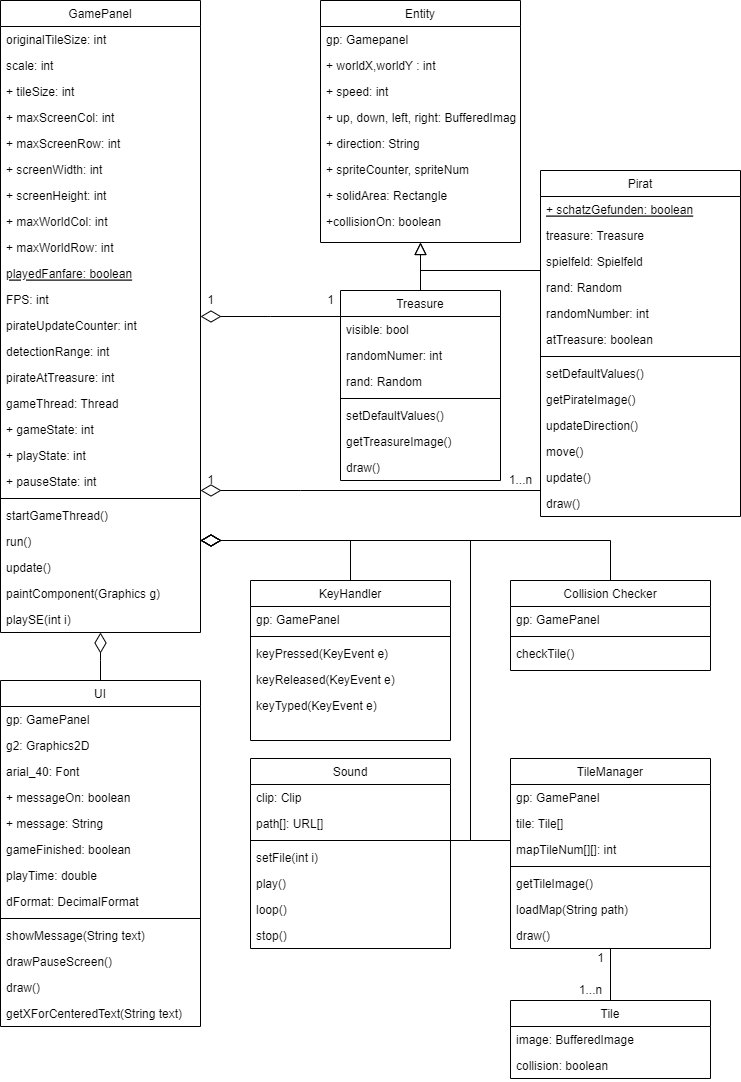
\includegraphics[scale=0.4]{bilder/UML_Klassendiagramm_Java.png}
  \label{fig:UML_Klassendiagramm_Java}       %fig:ID
  \caption[UML-Klassendiagramm für die Umsetzung in Java]{UML-Klassendiagramm für die Umsetzung in Java}    %Bildunterschrift
\end{figure}

Die zentrale Klasse des Spiels ist die Klasse GamePanel, sie ist das Fenster, in dem sich alles abspielt. In der Klasse Main wird ein Fenster erzeugt, in dem sich das GamePanel befindet. In dieser Klasse werden auch alle Einstellungen festgelegt, die Frames die pro Sekunde dargestellt und berechnet werden sollen, Fenstergröße, Skalierung, wie viele Piraten vorhanden sein sollen und weitere Einstellungen.  
Für die Entitäten im Spiel selber gibt es eine Überklasse, Entity, von der die anderen Klassen Pirat und Schatz abgeleitet werden.  
Zur Verwaltung des Spiels sind noch weitere Klassen notwendig.

\textbf{Verwaltungsklassen}
\begin{itemize}\vspace{-1em}
\setlength{\itemsep}{-1em}
	\item GamePanel: Wie oben erwähnt bestimmt sie das Spielfenster und die Einstellungen.
	\item KeyHandler: Implementiert den KeyListener aus der AWT-Bibliothek, der Tastatureingaben verarbeitet.
	\item TileManager und Tiles: Tiles sind die Spielfeldkacheln, sie stellen die Insel dar und verwalten das Laden der Kacheln aus den verschiedenen Bilddateien und der Kartendatei.
	\item UI (User Interface): Sie ist für den Text auf dem Bildschirm zuständig,
	\item Sound: Nutzt die Java Sound Bibliotheken, um Tondateien abzuspielen. In unserem Fall die Fanfare, wenn der Schatz gefunden wird.
	\item CollisionChecker: Überprüft, ob die Kacheln, auf die sich eine Entität zubewegt Kollision auslöst.
\end{itemize}

Es werden also alle Verwaltungsklassen in entsprechenden Objekten instanziiert, die Funktion zum Starten des Threads definiert. Hier wird auch der Status des Spiels festgelegt, um pausieren zu erlauben.

Moderne Prozessoren sind sehr schnell und können die Aktualisierung der Spielzustände und der Darstellung sehr schnell berechnen. Um das Spiel verfolgen zu können muss die Rate, mit der das Spiel dargestellt wird, begrenzt werden, siehe Listing \ref{lst:update}.

\begin{lstlisting}[language=Java, caption=Beschränkung der Aktualisierungen, label={lst:update}]
public void run() {
	double drawInterval = 1000000000/FPS;
	double delta = 0;
	long lastTime = System.nanoTime();
	long currentTime;
	
	while(gameThread!= null) {
		currentTime = System.nanoTime();
		delta += (currentTime - lastTime) / drawInterval;
		lastTime = currentTime;
		
		if(delta >=1) {
			update();
			repaint();
			delta--;
		}
	}
}
\end{lstlisting}

In der Funktion update() befindet sich die Logik des Spiels, dessen Auswirkungen im Anschluss mit der Funktion repaint() erneut gezeichnet werden.  
Die Details zu der Logik und allen weiteren Klassen sind im GitHub Repository zu sehen, siehe Notiz am Anfang des Abschnitts \ref{sec:Umsetzung_Java}.

Die Funktion update() überprüft zuerst in welchem Zustand sich das Spiel befindet. Mit derselben Logik wie in Listing \ref{lst:update} wird auch in der update() Funktion sichergestellt, dass die Piraten nur in bestimmten Zeitabständen ihre Richtung wechseln, dies geschieht in der update() Funktion der Klasse Pirat.
Wenn der Schatz jedoch gefunden wurde, bewegen sie sich kontinuierlich auf den Schatz zu.
Der Rest der Logik in dieser Funktion überprüft den Abstand jedes Piraten zum Schatz und setzt den Status der Piraten dem entsprechend, so dass sie sich nicht mehr bewegen, wenn sie am Schatz sind bzw. dass das Spiel zu Ende ist, wenn alle am Schatz sind und eine kleine Fanfare abgespielt wird.
  
  
Die repaint() Funktion ist eine Funktion der AWT-Bibliothek und sorgt dafür, dass die paintComponent() Funktion aufgerufen wird. Diese zeichnet abhängig vom Spielzustand die Entsprechenden Darstellungen auf den Bildschirm. Dafür wird hauptsächlich die Verwaltungsklasse UI in Anspruch genommen.



\section{Umsetzung in Unreal Engine}
\emph{Notiz: Der Quelltext der Umsetzung in Unreal ist auf \url{https://github.com/TheidenHD/Studienprojekt/} zu finden. \\
Das fertige Projekt ist auf \url{https://github.com/TheidenHD/Studienprojekt/releases/tag/1.0/} zu finden.}\\

Aufgrund der Komplexität von Unreal werden einige Standard-Klassen benötigt, die keinen großen Einfluss auf das Endprodukt haben. Beispiele sind hier der GameMode, welcher unter anderem zur Definition von Standardklassen und die GameInstance, welche hier zum Übermitteln von Variablen zwischen bestimmten Abschnitten im Projektablauf.

\subsection{UI}
Die Benutzeroberflächen werden aus einzelnen Bausteinen zusammengesetzt, die am Ende über das laufende Projekt gerendert werden. Wir verwenden dies im Hauptmenü, wo wir ein laufendes Level haben, damit wir einen animierten Hintergrund haben und im Pausemenü, wo wir die Ausführung des Levels pausieren, die Bewegungskontrolle deaktivieren und einen Unschärfe-Effekt über den Hintergrund legen. Das Klicken der Knöpfe erzeugt Events, die wir behandeln müssen, um den erwünschten Effekt zu erhalten.


\subsection{Level}
Das Projekt hat zwei Level, das Erste wird als Hintergrund für das Hauptmenü benutzt. In ihm befinden sich lediglich einige animierte Objekt und eine statische Kamera. Das Zweite ist das Spielfeld, in dem die Piraten nach dem Schatz suchen. Das Spielfeld ist statisch designt, das heißt, die Piraten starten immer an der gleichen Stell und der Schatz wird beim Start an einer von 6 vordefinierten Positionen zufällig platziert. Der Schatz kann hierbei unsichtbar sein, dies ändert allerdings nur die Sichtbarkeit für den Spieler und hat keinen Einfluss auf die Erkennbarkeit durch die Piraten und auf die Kollision. Die Piraten haben unterschiedliche Bewegungsgeschwindigkeiten, Blickwinkel und Sichtweiten. Diese werden in jeder Instanz durch Variablen definiert und nach dem Platzieren selbständig eingelesen und in den jeweiligen Komponenten hineingeschrieben. Außerdem verwendet eine Instanz das weibliche Modell und alle anderen das standard-männliche Modell.

\subsection{Künstliche Intelligenz}
Für die Künstliche werden 5 verschiedene Objekte verwendet. Vier davon sind für den Piraten und das fünfte ist der Schatz, den die Piraten suchen. Als erstes haben wir den Charakter, welcher alle physischen Komponenten beinhaltet, wie das Bewegungsmodul, die Sensorik und das Modell, welches für den Spieler sichtbar ist. Außerdem ist er für die Animation des Modells zuständig. Als zweites haben wir den Controller, welcher als Gehirn für den Piraten fungiert und alle Entscheidungen trifft. Als drittens haben wir einen Entscheidungsbaum, welcher ein Flowchart ist, für alle Entscheidungen des Controllers.  Und zu guter Letzt haben wir noch ein 
Blackboard, welches Variablen für den Entscheidungsbaum bereithält. Der Schatz hat keine besonderen Bestandteile und wird lediglich im Controller als Ziel für die Sensorik definiert.

\subsection{Sensorik}
Die Sensorik kann Ziele auf zwei unterschiedliche Methoden wahrnehmen, visuell und auditiv. Da wir hier nicht mit Geräuschen arbeiten, können wir den auditiven Teil einfach ignorieren. Beim visuellen Teil wird ein Kegel vom Kopf des Charakters aufgespannt und für alle Objekte der Klasse Pawn und deren Unterklassen, die sich in diesem Kegel befinden und nicht durch ein anderes undurchsichtiges Objekt verdeckt werden, wird ein Event ausgeworfen, in dem man nun überprüfen muss, ob dieses Objekt das Gesuchte ist.

\subsection{Bewegung}
Damit sich die Piraten bewegen können, benötigen wir zwei Komponenten, das Level, in dem der Pirat sich bewegt und das Bewegungsmodul im Piraten selbst. Damit er sich durch das Level bewegen kann, benötigt er mindestens eine Fläche und eine Definition, welche der Flächen begehbar sind. Diese Definition ist das \gls{NavMesh}, welches dynamisch durch das NavMeshBoundsVolume im laufenden Betrieb erstellt wird. Wenn sich der Pirat nun im \gls{NavMesh} befindet und einen Punkt bekommt, der sich ebenfalls im \gls{NavMesh} befindet, wird er sich auf den kürzesten Weg zu diesem Punkt bewegen.

\subsection{Ablauf}
Wenn die Piraten auf dem Level erscheinen, überprüfen sie zuerst, ob der Schatz bereits gefunden wurde. Wenn dies der Fall ist, gehen sie zum Schatz und ignorieren alles andere. Wenn dies nicht der Fall ist, suchen sie sich einen zufälligen Punkt in einem bestimmten Radius, zu dem sie sich bewegen können und gehen dann zu ihm. Während der Bewegung halten die Piraten Ausschau nach dem Schatz und wenn sie ihn finden, bleiben sie sofort stehen, holen sich vom Level eine Liste von allen Instanzen derselben Klasse und benachrichtigen diese, dass der Schatz gefunden wurde und wo er sich befindet.
Diese Funktion befindet sich in einer Endlosschleife, die entweder nach dem Erreichen des Punktes oder dem Finden des Schatzes von vorne beginnt.

\section{Umsetzung in Unity Engine}
\emph{Notiz: Das Unity Projekt ist auf \url{https://github.com/SvenGamerTV/Studienprojekt.git} zu finden.} \\
\subsection{Grundlagen}
In diesem Abschnitt werden einige essentielle Begriffe geklärt, welche für das Verständnis der folgenden Abschnitte benötigt wird.
\subsubsection{GameObjects}
Ein GameObject in der Unity Engine ist das zentralste Element eines Projektes. Als GameObjects werden alle im sich im Projekt befindlichen Inhalte verstanden, also jedes Objekt, jede Figur, jede Szene und auch z.B. die Kamera sowie die Belichtungsquellen sind GameObjects. Jedes dieser GameObjects hat eigene Eigenschaften, welche für jedes GameObject individuell bestimmt werden. Ein GameObject selbst besitzt jedoch keine Funktionalität, sondern stellt nur ein Modell oder z.B. eine Lichtquelle innerhalb des Projektes dar. Damit ein GameObject mit dem Rest des Projektes oder anderen GameObject interagieren kann muss dem GameObject ein Skript o.Ä. zugewiesen werden.

\subsubsection{Skripte}
Skripte ermöglichen den GameObject die Interaktion miteinander und mit dem Rest des Projektes. Die gesamte Programmlogik eines Projektes ist in einem oder mehreren Skripten hinterlegt. Skripte können mit anderen Skripten interagieren, je nach Freigabe der einzelnen Funktionen, welche in der Skripten sind. Skripte können zudem auch mit den GameObjects interagieren und u.A. deren Eigenschaften abrufen oder verändern. Hierzu kann ein Skript einem GameObject zugewiesen werden und auf die aktuelle Instanz somit zugreifen oder von außen auf eine bestimmte Instanz einwirken. Bei der Zuweisung von Skripte ist ein Skript nicht an ein einzelnes Objekt gebunden, sondern ein Skript kann beliebig vielen GameObjects zugewiesen werden. Genauso kann einem einzelnen GameObject auch eine beliebige Anzahl an Skripten zugewiesen sein.

\subsubsection{Prefabs}
Ein Prefab ist ein Pre-Fabricated-Object, also ein GameObject, welches u.A. bereits Skripte, Texturen oder Audio-Datei zugewiesen bekommen hat und somit als fertige Figur, Terrainstruktur oder Ähnliches in das Projekt eingebunden werden kann. Prefabs können beliebig oft innerhalb eines Projektes verwendet werden. Jede neue Einbindung eines Prefabs erzeugt eine neue Instanz, welche entweder vom Entwickler selbst oder durch ein Skript angesteuert und bearbeitet werden können. Dabei nimmt die Änderung an einer Instanz eines Prefabs keinerlei Einfluss auf die restlichen Instanzen.

\subsection{Objektorientierte Programmierung in Unity}
Durch die Strukturierung der einzelne Projektelemente in GameObjects und die Instanziierung der GameObjecte arbeitet die Unity Engine objektorientiert. Jedes einzelne GameObject ist hierbei vergleichbar mit z.B. einer Klasse in Java, welche ebenfalls über bestimmte Eigenschaften verfügt, welche bei der Instanziierung bei Objekten des gleichen Modells unterschiedlich aussehen können und jede Instanz unabhängig der anderen agiert. Nach diesem Modell arbeitet auch die Unity Engine. Hier besitzt jedes GameObject einen eigenen Satz Eigenschaften, welche bearbeiten werden können, ohne dass gleich Objekte davon beeinflusst werden.

\subsection{Realisierung der Anforderungen}
\subsubsection{Bewegung der Piraten}
Die Piraten sollen sich nach einem zufälligen Muster über das Spielfeld bewegen, ohne wiederum bereits besuchte Position wieder zu betreten. hierzu muss konstant eine neue Position für jeden der Piraten erstellt werden. Diese Position muss innerhalb des Spielbereiches liegen und darf vom Piraten vorher noch nicht besucht worden sein. Um dies sicherzustellen, muss daher jeder Pirat über eine sich nach jeder Bewegung erweiternde Liste verfügen, welche die Position, die der Pirat hat, speichert und bei zukünftigen Bewegungen immer überprüft, ob die Position sich mit einer, welche bereits in der Liste ist, deckt. Ist dies der Fall oder die Position würde außerhalb des Spielbereiches liegen, dann wird so lange eine neue Position generiert, bis eine Position gefunden wurde, welche alle Bedingungen erfüllt. Als letztes wird geprüft, ob sich bereits ein Pirat in der Nähe des Schatzes befindet. Ist dies gegeben, dann wird die Position für alle Piraten auf dem Feld auf die des Schatzes gesetzt und die Piraten bewegen sich zum Schatz. Die Ansteuerung aller Piraten ist in diesem Fall möglich da jedem Objekt in Unity ein Tag zugewiesen werden kann, über welchen dann durch eine Methode eine Liste aller Objekte erstellt werden kann, welche dann in diesem Fall nur Objekt mit dem Tag Pirat enthält. Wird nun über diese Liste iteriert, können Methoden für alle Piraten ausgeführt werden. Wenn der Schatz gefunden wurde, wird die Generierung von neuen Positionen gestoppt und dementsprechend bewegen sich die Piraten nicht mehr vom Schatz weg. 

\subsubsection{Änderung der Sichtbarkeit des Schatzes}
Die Sichtbarkeit des Schatzes soll von zwei Faktoren beeinflusst werden, zum einen durch einen Input vom Spieler und zum anderen durch das Finden des Schatzes durch einen der Piraten. Für den Ersten Fall muss dem Spieler die Möglichkeit geschaffen werden mit dem Spiel zu interagieren. Hierzu wird ein ButtonTrigger verwendet, also wird eine Aktion ausgeführt, sobald der Spieler eine Taste drückt. In dieser Implementation wird die Sichtbarkeit des Schatzes über die Taste V gesteuert. Drückt der Spieler also die V- Taste wird der Schatz unsichtbar oder sichtbar je nach dem, was vorher vorgelegen hat. Dies geschieht innerhalb der Update- Methode des Skriptes, welches die Aktionen des Schatzes steuert. Diese Update-Methode wird jeden Tick erneut abgerufen und garantiert somit das der Tastendruck des Nutzers auch erkannt und verarbeitet werden kann, dies Geschieht über eine in der Unity Engine erhaltene Methode Input.KeyUp(KeyCode) diese erfasst in einem Boolean-Wert, ob die als KeyCode angegebene Taste wieder losgelassen wurde. Ist dieser Wert True wird der Renderer, also die Komponente des Schatzes, welche das Modell in 3D auf dem Spielfeld anzeigt, deaktiviert bzw. aktiviert, sollte er vorher deaktiviert worden sein. Zuletzt wird in der Update-Methode erfasst, ob der Schatz bereits gefunden wurde, wenn dies der Fall ist, wird der Renderer aktiv gesetzt und der Einfluss des Tastendrucks wird vom Spiel nicht mehr berücksichtigt, sodass der Schatz, nachdem er gefunden wurde, immer sichtbar bleibt.


\chapter{Ergebnisse}
Die Untersuchung der verschiedenen Methoden zur Erstellung eines Spiels in verschiedenen Umgebungen hat ergeben, dass vorgefertigte Umgebungen und Engines viel Aufwand ersparen können. So werden viele Managementklassen schon vorgefertigt ausgeliefert und müssen nicht selbst erstellt werden. Auch deren Logik besteht zum größten Teil schon und kann nach Bedarf modifiziert werden.  
Diese Rationalisierung durch die angepassten Umgebungen ermöglichen einen schnellen Einstieg in die Entwicklung von neuen Projekten und senkt auch erheblich die Hürde, um in diese Form der Softwareentwicklung einzusteigen.

Die Entwicklung und Auslieferung auf verschiedene Plattformen werden ebenfalls erheblich vereinfacht.

Auch die Tatsache, dass die meisten bekannten Werkzeuge beziehungsweise Plattformen kostenlos erhältlich sind, spricht für die Auswahl einer dieser Umgebungen. Weiterhin wird durch die weite Verbreitung und Erhältlichkeit dafür gesorgt, dass es viele Anleitungen, Unterstützung, Beispiele und auch Ressourcen wie Modelle, Musik und Effekte zur Verfügung stehen.

\chapter{Fazit}
In diesem Studienprojekt wurde zuerst betrachtet unter welchen Bedingungen Spiele entwickelt werden können. Als Grundlage dient die \gls{OOP}, dessen grundlegende Kerneigenschaften betrachtet wurden.
Anschließend wurden drei verschiedene Umgebungen für die Entwicklung des Prototyps erörtert.  
Ein möglicher Punkt der Verbesserung könnte es sein, weitere Umgebungen zu betrachten, da sich diese eventuell doch erheblicher voneinander unterscheiden als angenommen.  
  
Es wurde ein kleiner Überblick über die verwendeten Werkzeuge geschaffen und die Anforderungen an das Spiel formuliert. Daraufhin dann die Realisierung in den verschiedenen Umgebungen aufgebrochen und beschrieben.


\chapter{Ausblick}
Dieses Projekt könnte noch erweitert werden, indem neue oder komplexere Anforderungen gestellt und untersucht werden. Auch könnte die Untersuchung der Umgebungen erweitert werden, indem weitere in Frage kommende Umgebungen betrachtet und verglichen werden.  
  
Andererseits wäre es auch möglich weiter zu erörtern, inwiefern Simulationen zur Untersuchung von anderen Gegebenheiten sinnvoll sind und ob diese vergleichbare Ergebnisse liefern. Zum Beispiel könnte untersucht werden, wie sich verschiedene Suchmuster für die Piraten bei der Suche nach dem Schatz auswirken und welche am effektivsten sind.

%%% Codesnippets

%% Liste
%\textbf{Grundwerte}
%\begin{itemize}\vspace{-1em}
%\setlength{\itemsep}{-1em}
%	\item \textbf{Integrität}: Die Daten oder das System sind nicht von Unbefugten veränderbar. Alle Änderungen müssen nachvollziehbar sein.
%	\item \textbf{Vertraulichkeit}: Die Daten dürfen nur von autorisierten Personen abgerufen und verändert werden. Dies gilt sowohl für gespeicherte Dateien, als auch die Datenübertragung.
%	\item \textbf{Verfügbarkeit}: Die Daten und Systeme müssen erreichbar sein. Systemausfälle müssen vermieden werden. Wenn man eine Verfügbarkeit von "four nines" (99.99\% der Zeit) gewährleisten möchte, dann sind z.B. nur Ausfälle für 52:36 Minuten pro Jahr vertretbar.
%\end{itemize}

%% Bild
%\begin{figure}[H]
%  \centering
%  \includegraphics[scale=0.5]{bilder/Netzplan.JPG}
%  \label{fig:kernabsicherung}       %fig:ID
%  \caption[Beispielhafter Netzplan nach BSI 200-2]{\cite{BSI200_2} Seite 90: Auszug aus dem bereinigten Netzplan der RECPLAST GmbH (Teilausschnitt)}    %Bildunterschrift
%\end{figure}


%% Code
%\begin{lstlisting}[language=csh, caption=Python example]
%public async Task<IActionResult> Archiv()
%    {
%        string UserPersId = User.Identity?.Name ?? "Empty";
%
%        return View(await _context.Dokumente.Where(x => x.PersonalNummer == UserPersId).ToListAsync());
%    }
%//test
%\end{lstlisting}


%%%%%%%%%%%%%%%%%%%%%%%%%%
% Quellen
%%%%%%%%%%%%%%%%%%%%%%%%%

\bibliography{literatur}

\bibliographystyle{hwrbib}
%% \bibliographystyle{alpha} %% tu es nicht, niemals, das ist eklig, nicht einkommentieren

\chapter*{Ehrenwörtliche Erklärung}
\addcontentsline{toc}{chapter}{Ehrenwörtliche Erklärung}

% Keine Kopf- und Fußzeilen ausgeben
\thispagestyle{empty}
% Aber trotzdem ins Inhaltsverzeichnis aufnehmen
%\addcontentsline{toc}{section}{Eidesstattliche Erklärung}

% Hier der offizielle Text der eidesstattlichen Erklärung
Ich erkläre ehrenwörtlich:
\begin{enumerate}
	\item dass ich meine Bachelor-Thesis selbstständig verfasst habe,
	\item dass ich die Übernahme wörtlicher Zitate aus der Literatur sowie die Verwendung der Gedanken anderer Autoren an den entsprechenden Stellen innerhalb der Arbeit gekennzeichnet habe,
	\item dass ich meine Bachelor-Thesis bei keiner anderen Prüfung vorgelegt habe.
\end{enumerate}
Ich bin mir bewusst, dass eine falsche Erklärung rechtliche Folgen haben wird.
% Etwas Abstand für die Unterschrift
\vspace{2cm}

% Hier kommt die Unterschrift drüber
\begin{tabular}{lp{4em}l} 
 \hspace{5cm}   && \hspace{6cm} \\\cline{1-1}\cline{3-3} 
 Ort, Datum     && \studentNameEins \\ [10ex]
 \hspace{5cm}   && \hspace{6cm} \\\cline{1-1}\cline{3-3} 
 Ort, Datum     && \studentNameZwei \\ [10ex]
 \hspace{5cm}   && \hspace{6cm} \\\cline{1-1}\cline{3-3} 
 Ort, Datum     && \studentNameDrei \\ [10ex]
\end{tabular}

\end{document}

